% SIAM Supplemental File Template
\documentclass[final,supplement,onefignum,onetabnum]{siamonline171218}


\usepackage{subfigure}
\usepackage{graphicx}
\usepackage{amsmath}

% SIAM Shared Information Template
% This is information that is shared between the main document and any
% supplement. If no supplement is required, then this information can
% be included directly in the main document.


% Packages and macros go here
\usepackage{lipsum}
\usepackage{amsfonts}
\usepackage{graphicx}
\usepackage{epstopdf}
\usepackage{algorithmic}
\ifpdf
  \DeclareGraphicsExtensions{.eps,.pdf,.png,.jpg}
\else
  \DeclareGraphicsExtensions{.eps}
\fi

% Prevent itemized lists from running into the left margin inside theorems and proofs
\usepackage{enumitem}
\setlist[enumerate]{leftmargin=.5in}
\setlist[itemize]{leftmargin=.5in}

% Add a serial/Oxford comma by default.
\newcommand{\creflastconjunction}{, and~}

% Used for creating new theorem and remark environments
\newsiamremark{remark}{Remark}
\newsiamremark{hypothesis}{Hypothesis}
\crefname{hypothesis}{Hypothesis}{Hypotheses}
\newsiamthm{claim}{Claim}

% Sets running headers as well as PDF title and authors
\headers{SCENE-Net}{D. Lavado, C. Soares, and A. Micheletti}

% Title. If the supplement option is on, then "Supplementary Material"
% is automatically inserted before the title.
\title{
Low-Resource White-Box Semantic Segmentation of Supporting Towers on 3D Point Clouds via Signature Shape Identification
    % \thanks{Submitted to the editors DATE.
    %     \funding{This work was funded by the Fog Research Institute under contract no.~FRI-454.}
    % }
}



\author{Diogo Lavado\footnotemark[1], Cláudia Soares\thanks{NOVA School of Science and Technology, Lisbon 
  (\email{d.lavado@campus.fct.unl.pt}, \email{claudia.soares@fct.unl.pt}).}
\and Alessandra Micheletti\footnotemark[2], Giovanni Bocchi\thanks{University of Milan, Milan
  (\email{alessandra.micheletti@unimi.it}, \email{giovanni.bocchi1@unimi.it}).}
\and Alex Coronati\footnotemark[3], Manuel Pio\thanks{EDP NEW, Lisbon
  (\email{alex.coronati@edp.pt}, \email{manuelpio.silva@edp.pt}).}
\and Patrizio Frosini\thanks{University of Bologna, Bologna
  (\email{patrizio.frosini@unibo.it}).}
}
% \author{Dianne Doe\thanks{Imagination Corp., Chicago, IL 
%   (\email{ddoe@imag.com}, \url{http://www.imag.com/\string~ddoe/}).}
% \and Paul T. Frank\thanks{Department of Applied Mathematics, Fictional University, Boise, ID 
%   (\email{ptfrank@fictional.edu}, \email{jesmith@fictional.edu}).}
% \and Jane E. Smith\footnotemark[3]}

\usepackage{amsopn}
\DeclareMathOperator{\diag}{diag}


%%%% HELPER CODE FOR DEALING WITH EXTERNAL REFERENCES ON OVERLEAF
% (from an answer by cyberSingularity at http://tex.stackexchange.com/a/69832/226)
%%%
\makeatletter
\newcommand*{\addFileDependency}[1]{% argument=file name and extension
  \typeout{(#1)}% latexmk will find this if $recorder=0 (however, in that case, it will ignore #1 if it is a .aux or .pdf file etc and it exists! if it doesn't exist, it will appear in the list of dependents regardless)
  \@addtofilelist{#1}% if you want it to appear in \listfiles, not really necessary and latexmk doesn't use this
  \IfFileExists{#1}{}{\typeout{No file #1.}}% latexmk will find this message if #1 doesn't exist (yet)
}
\makeatother

\newcommand*{\myexternaldocument}[1]{%
    \externaldocument{#1}%
    \addFileDependency{#1.tex}%
    \addFileDependency{#1.aux}%
}
%%% END HELPER CODE

%%% Local Variables: 
%%% mode:latex
%%% TeX-master: "ex_article"
%%% End: 


%% Use \myexternaldocument on Overleaf
\myexternaldocument{ex_article}

% Optional PDF information
\ifpdf
\hypersetup{
  pdftitle={Supplementary Materials: An Example Article},
  pdfauthor={D. Doe, P. T. Frank, and J. E. Smith}
}
\fi

\begin{document}

\maketitle

\section{TS40K Dataset\label{sec:ts40k}}

Electrical companies are responsible for the maintenance and inspection of the transmission system. They deploy low-flying helicopters to scan rural environments, from a BEV perspective, where the electrical grid is located.
%
The produced point clouds exhibit different data properties when compared to 3D scenes captured from other viewpoints, such as from a vehicle.
Namely, they show high point density and no object occlusion, scene elements present homogeneous density and no sparsity.
%
Then, the acquired 3D data is processed by maintenance personnel. Specifically, as the raw point clouds are dense and mainly encompass rural areas, data is sectioned into strips of land focused on the transmission system (Figure~\ref{fig:results}). 
%
\begin{figure*}
    \centering
    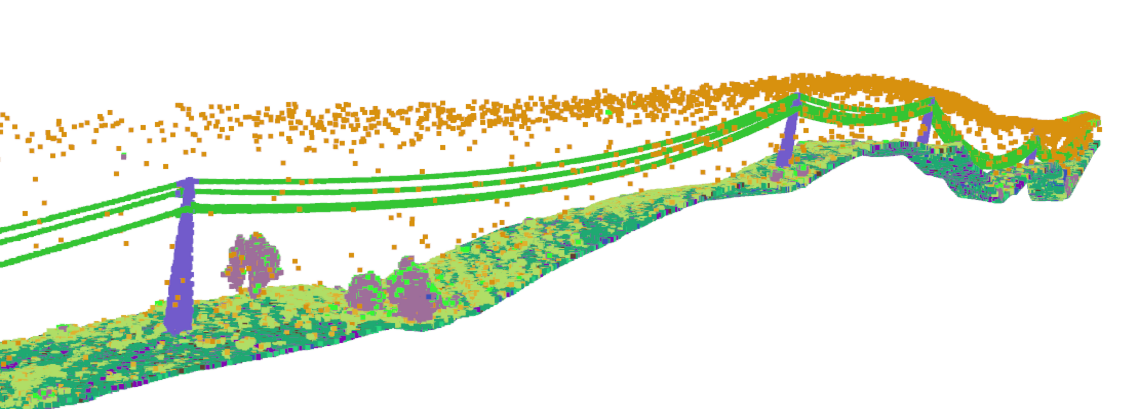
\includegraphics[width=1\linewidth]{data5-5.png}
    \caption{Visualization of TS40K raw point cloud with colored labels.}
    \label{fig:ts40k}
\end{figure*}
The raw data comprises several LiDAR files containing roughly 40 000 kilometers of the above land strips. 3D points therein are labeled with one out of 22 possible classes, such as power lines and their supporting towers, low and medium vegetation, rivers, railroads, human-made structures that do not belong to the transmission network, the ground, and optic cables, among others.
%
Table~\ref{tab:ts40k_labels} depicts these classes and their density in the dataset. Rail lines and road surfaces constitute the majority of the dataset (63\%), whereas classes of interest, such as power line supporting towers, make up less than 5\% of the overall data. 

\begin{table}[]
\caption{Available classes in the TS40K dataset and their distribution. Rail lines and road surfaces constitute the majority of the dataset (63\%). Our class of interest, power line towers, only makes up 0.52\%. 
Moreover, around 40\% of the tower points are mislabelled.\\}
\resizebox{\linewidth}{!}{%
\begin{tabular}{lll|lll}
\hline
\textbf{Label} &
  \textbf{Class} &
  \textbf{Density(\%)} &
  \textbf{Label} &
  \textbf{Class} &
  \textbf{Density(\%)} \\ \hline
0  & Created          & 0               & 11 & Road surface                    & \textbf{18.758} \\
1  & Unclassified     & 0.571           & 12 & Overlap points                  & 23.403          \\
2  & Ground           & 0.529           & 13 & Medium Reliability              & 0               \\
3  & Low vegetation   & 0.681           & 14 & Low Reliability                 & 0               \\
4 &
  Medium vegetation &
  0.241 &
  {\color[HTML]{CB0000} 15} &
  {\color[HTML]{CB0000} Power line support tower} &
  {\color[HTML]{CB0000} \textbf{0.519}} \\
5  & Natural obstacle & 1.069           & 16 & Main power line                 & 0.907           \\
6  & Human structures & 0               & 17 & Other power line                & 0.002           \\
7  & Low point        & 0.362           & 18 & Fiber optic cable               & 0               \\
8  & Model key points  & 0               & 19 & Not rated object to be consider & 8.205           \\
9  & Water            & 0               & 20 & Not rated object to be ignored  & 0               \\
10 & Rail             & \textbf{44.752} & 21 & Incidents                       & 0               \\ \hline
\end{tabular}%
}
\label{tab:ts40k_labels}
\end{table}


\subsection{Qualitative Results.}

In Figure~\ref{fig:results}, we can analyze the qualitative results on the TS40K dataset~(a) of SCENE-Net~(c) against a CNN is similar architecture as baseline~(b).
Even though the CNN achieves a higher Recall on the majority of the samples, it classifies most vertical scene elements as towers, which ultimately leads to a poor segmentation of supporting towers.
In contrast, SCENE-Net segments the body of towers and rejects other vertical objects that do not exhibit the prior knowledge encoded in the model.


\begin{figure*}[t]
\centering
\setkeys{Gin}{width=\textwidth}
    \addtocounter{subfigure}{-1}
    \subfigure{
    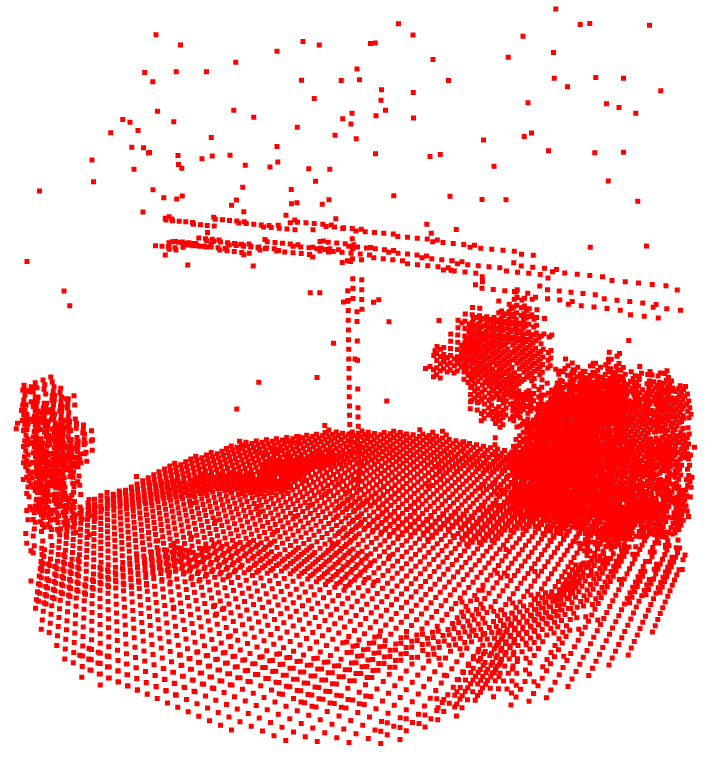
\includegraphics[width=.28\textwidth]
    {s33.png}}
    %
    \addtocounter{subfigure}{-1}
    \subfigure{
    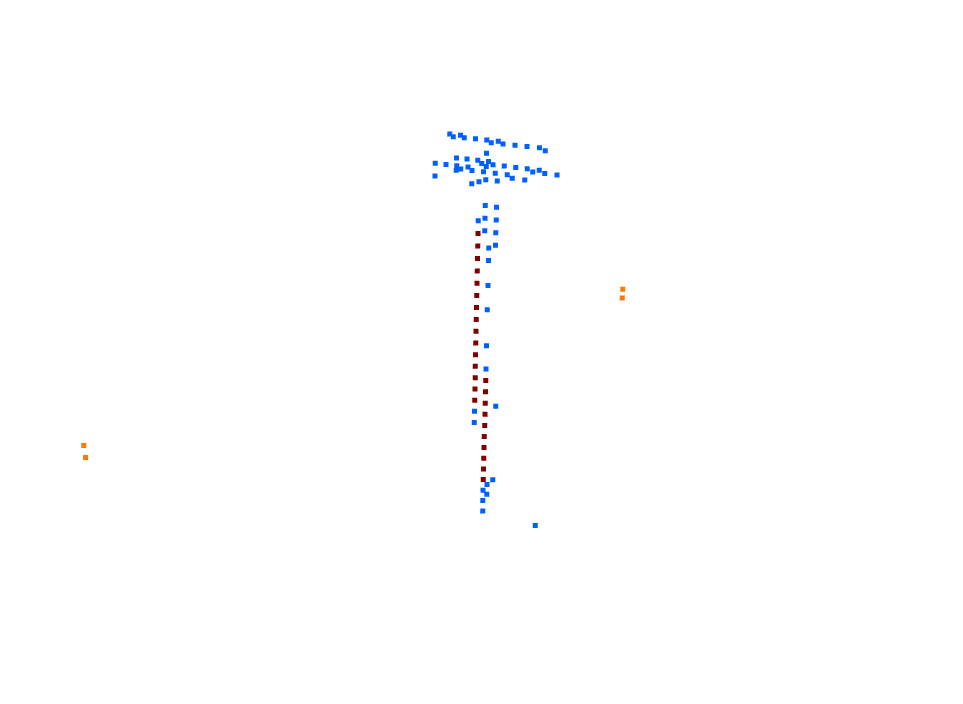
\includegraphics[width=.3\textwidth]{gnet_s33.png}}
    %
    \addtocounter{subfigure}{-1}
    \subfigure{
    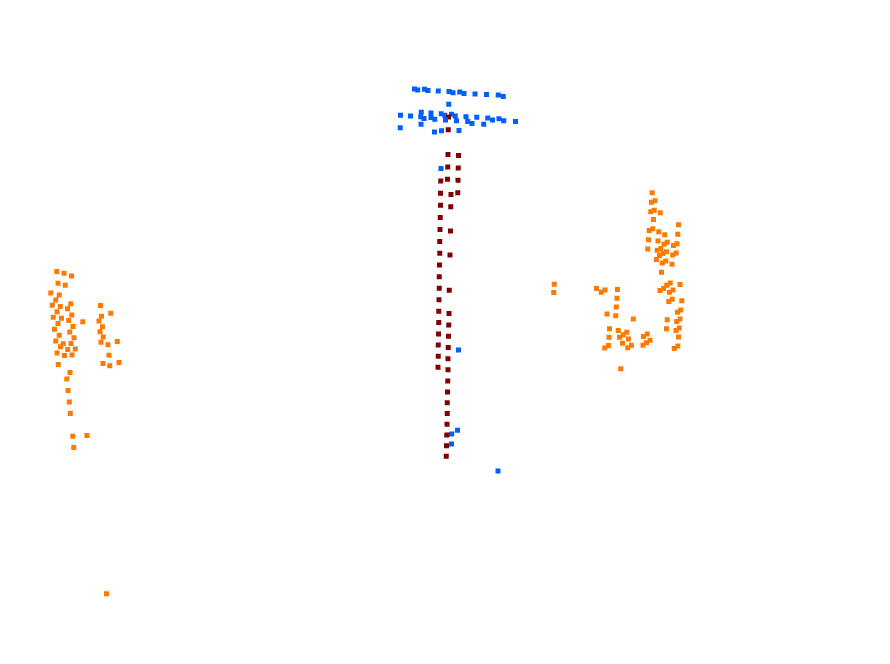
\includegraphics[width=.3\textwidth]{cnn_s33.png}}
    
    \addtocounter{subfigure}{-1}
    \subfigure{
    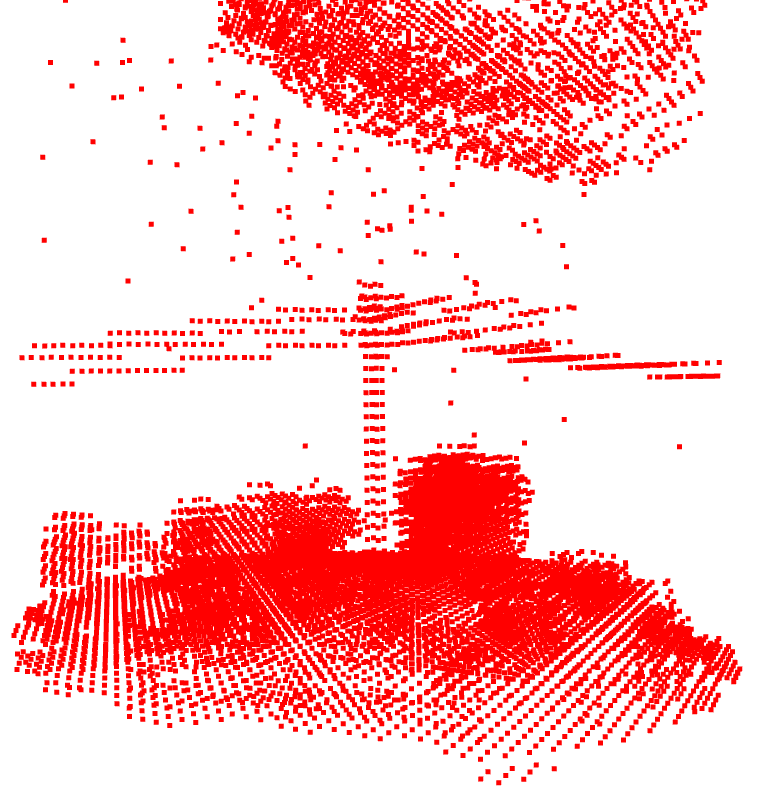
\includegraphics[width=.28\textwidth]
    {s34.png}}
    %
    \addtocounter{subfigure}{-1}
    \subfigure{
    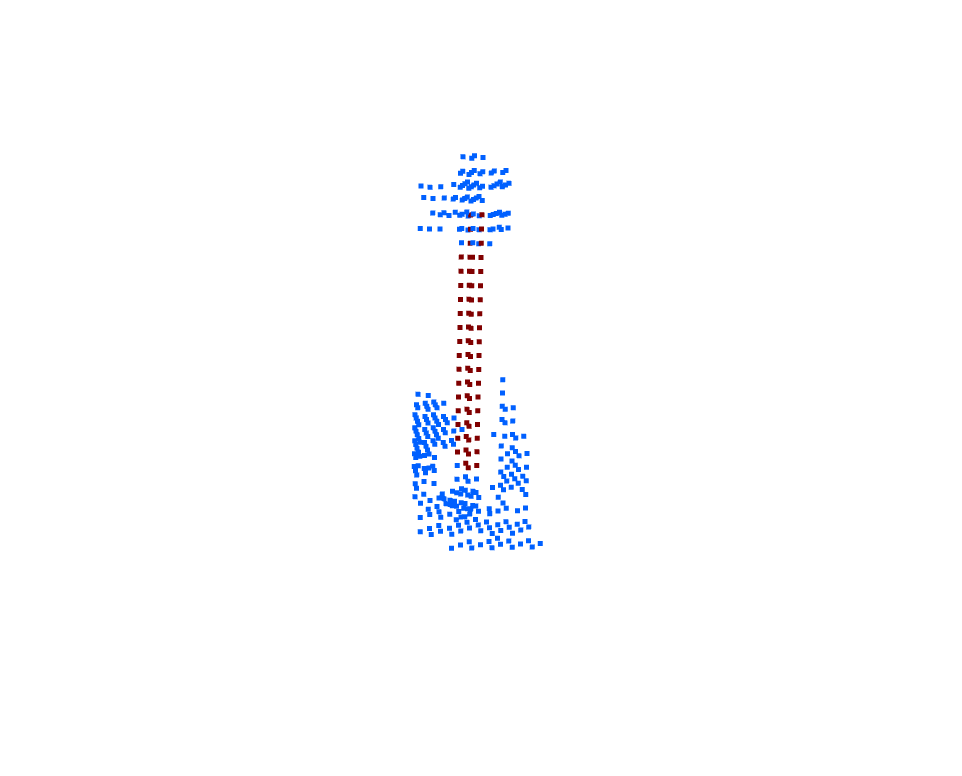
\includegraphics[width=.3\textwidth]{gnet_s34.png}}
    %
    \addtocounter{subfigure}{-1}
    \subfigure{
    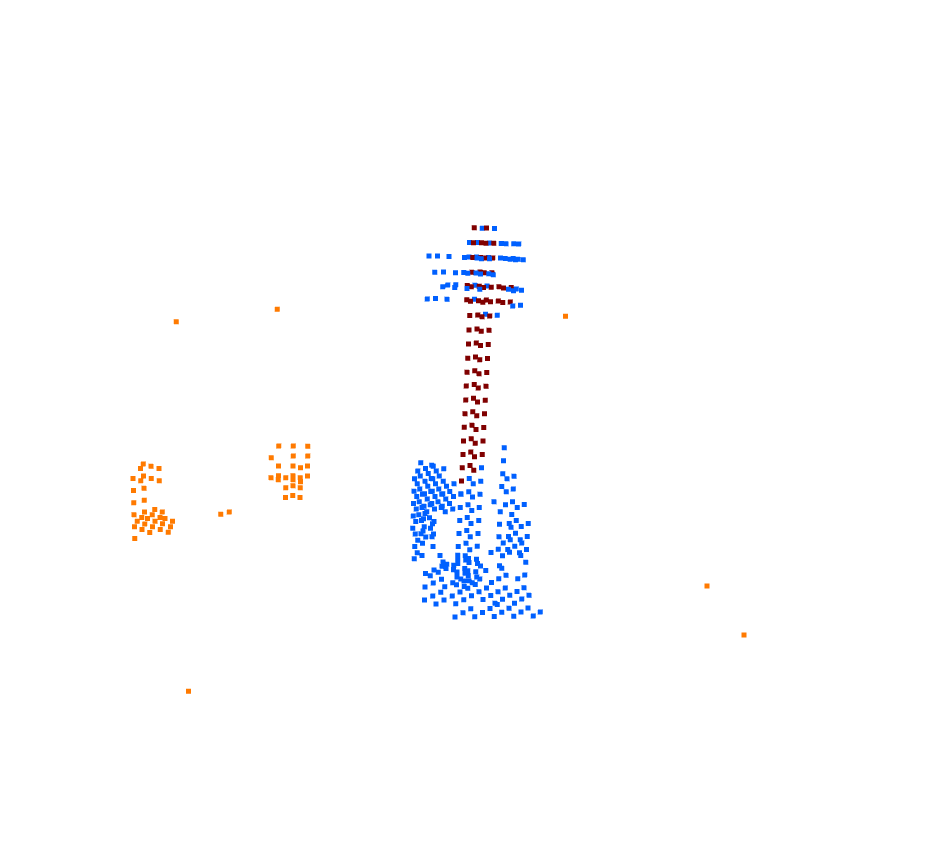
\includegraphics[width=.3\textwidth]{cnn_s34.png}}

    \addtocounter{subfigure}{-1}
    \subfigure{
    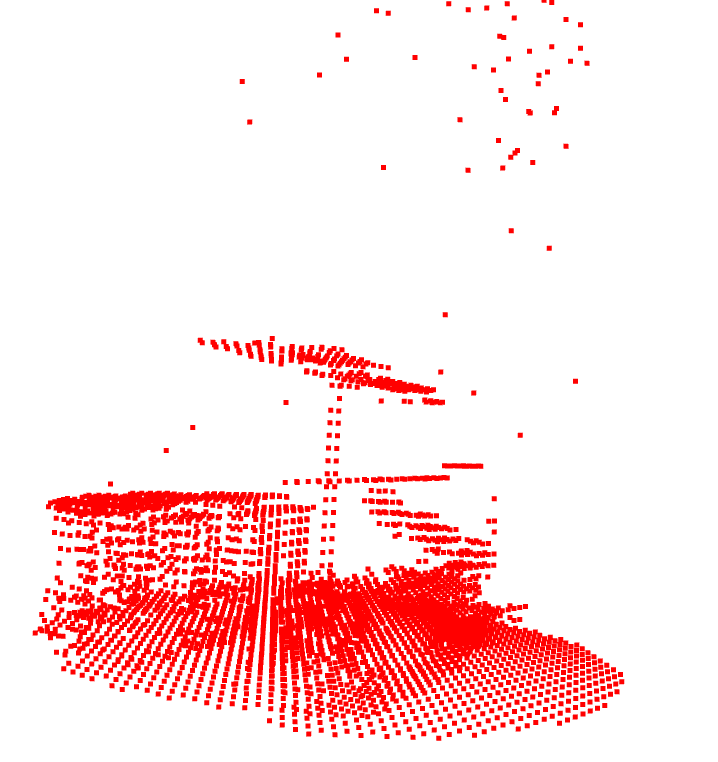
\includegraphics[width=.28\textwidth]
    {s41.png}}
    %
    \addtocounter{subfigure}{-1}
    \subfigure{
    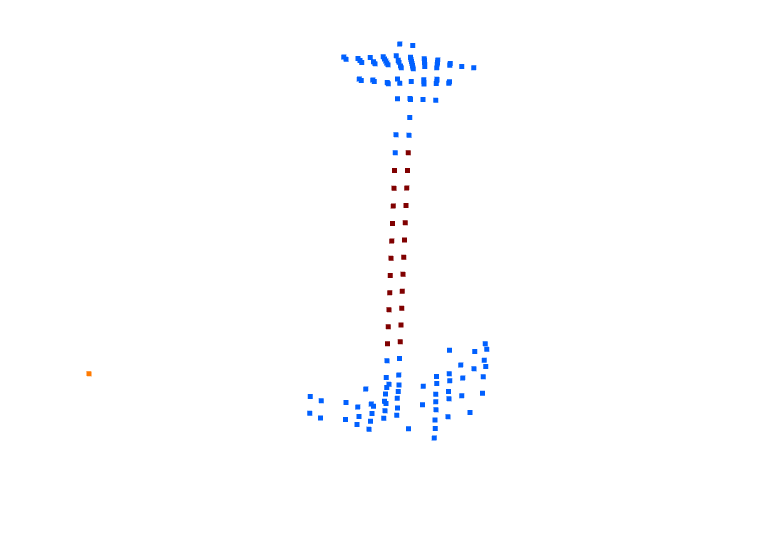
\includegraphics[width=.3\textwidth]{gnet_s41.png}}
    %
    \addtocounter{subfigure}{-1}
    \subfigure{
    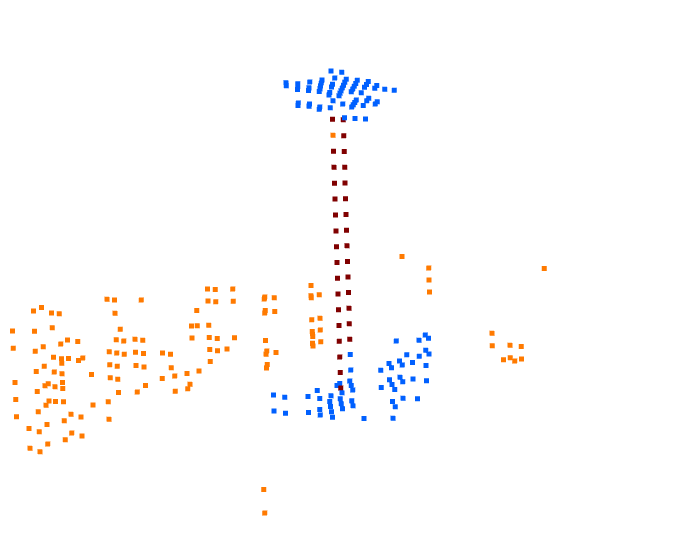
\includegraphics[width=.3\textwidth]{cnn_s41.png}}

    
    \subfigure[TS40K Sample]{
    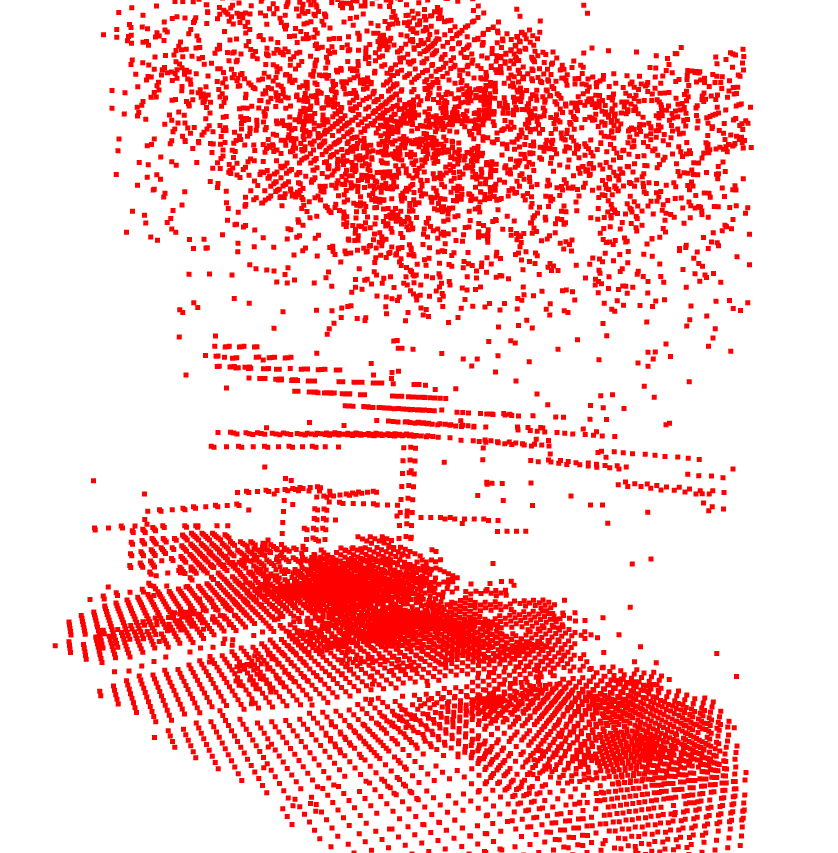
\includegraphics[width=.3\textwidth]
    {s36.png}}
    %
    \subfigure[SCENE-Net]{
    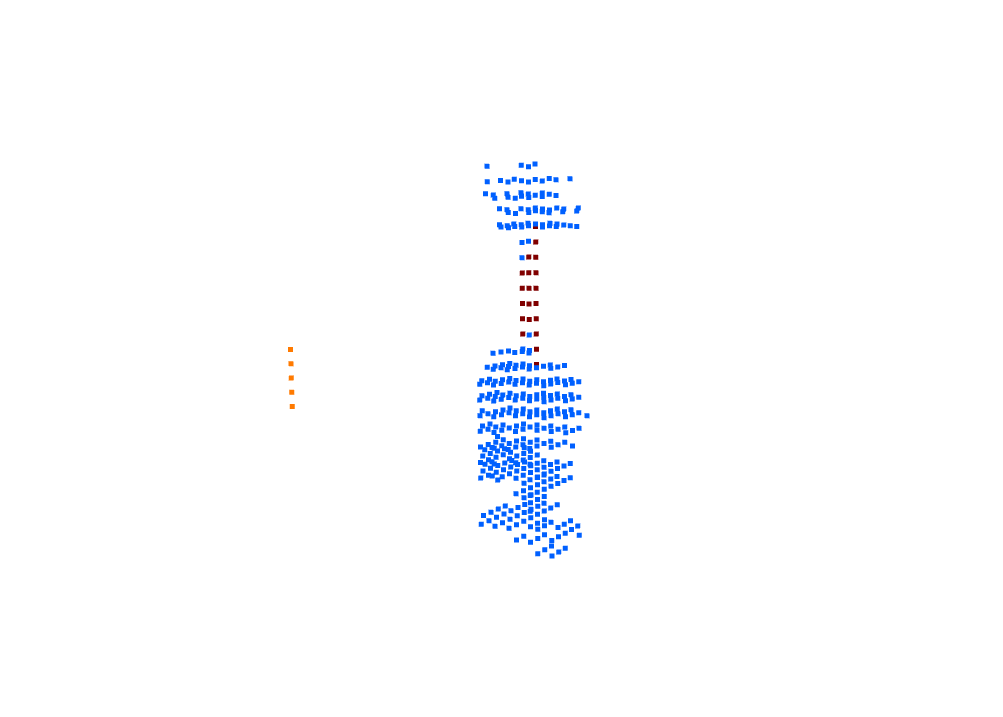
\includegraphics[width=.3\textwidth]{gnet_s36.png}}
    %
    \subfigure[CNN Baseline]{
    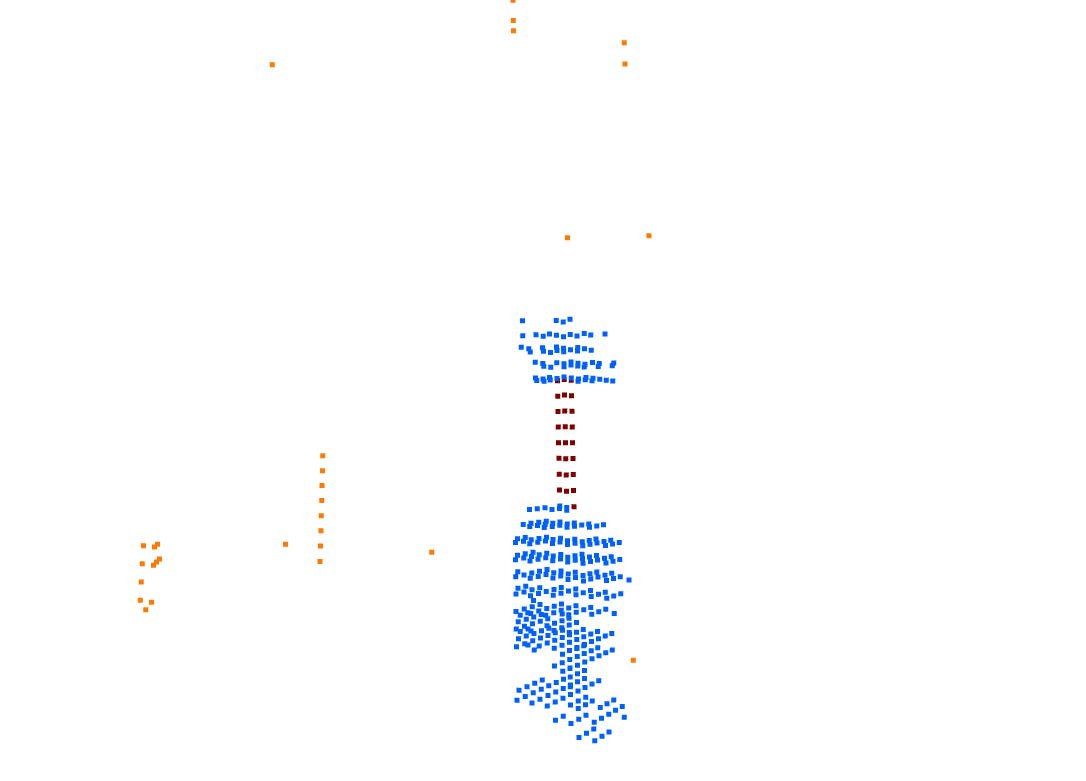
\includegraphics[width=.3\textwidth]{cnn_s36.png}}

    \subfigure{
    
\includegraphics[width=.5\columnwidth]
    {color_code_v2.pdf}}

    \caption{Qualitative results of SCENE-Net on the testing set of TS40K, against a CNN with similar architecture. Note that, in the last example, SCENE-Net clearly identifies a second unlabeled tower, whereas CNN identifies both the second tower and vegetation as towers.}
\label{fig:results}
\end{figure*}


\end{document}
